\section{Recurrent Neural Network}

\subsection{Hyperparameter Optimization}

This section explores the architecture of \glspl{rnn} tailored for our task. RNNs excel in processing sequential data,
making them an intuitive architectural choice under the assumption that the ordered eigenvalues should contain ``temporal'' information.\\
The section aims to investigate various architectural choices, including cell type, sequence order, and bidirectionality, to identify the
most effective configuration for the task at hand. \\
The iterative application of the same weights across sequence elements aligns well with the potential goal of using the
model in an \gls{fpga} implementation, where weight sharing can lead to significant efficiency gains.\\

Since a detailed theoretical introduction to \glspl{rnn} would be helpful for the following consideration of the effects of
certain RNN specific architecture decisions, but would
exceed the scope of this work, we refer to the literature~\cite[Chapter 10.2 ff.]{dlbook} for a comprehensive introduction to
\glspl{rnn} or to~\cite{dlcheatsheet} for a more compact overview.\\

\subsubsection{Selection of the RNN Cell Type}

Among the various \gls{rnn} cell types, the classic \gls{rnn} cell was chosen over \gls{lstm} and \gls{gru} cells. This
decsision will be substantiated through the combination of empirical findings and theoretical considerations, which will
be presented in this section.\\

\begin{figure}[H]
    \centering
    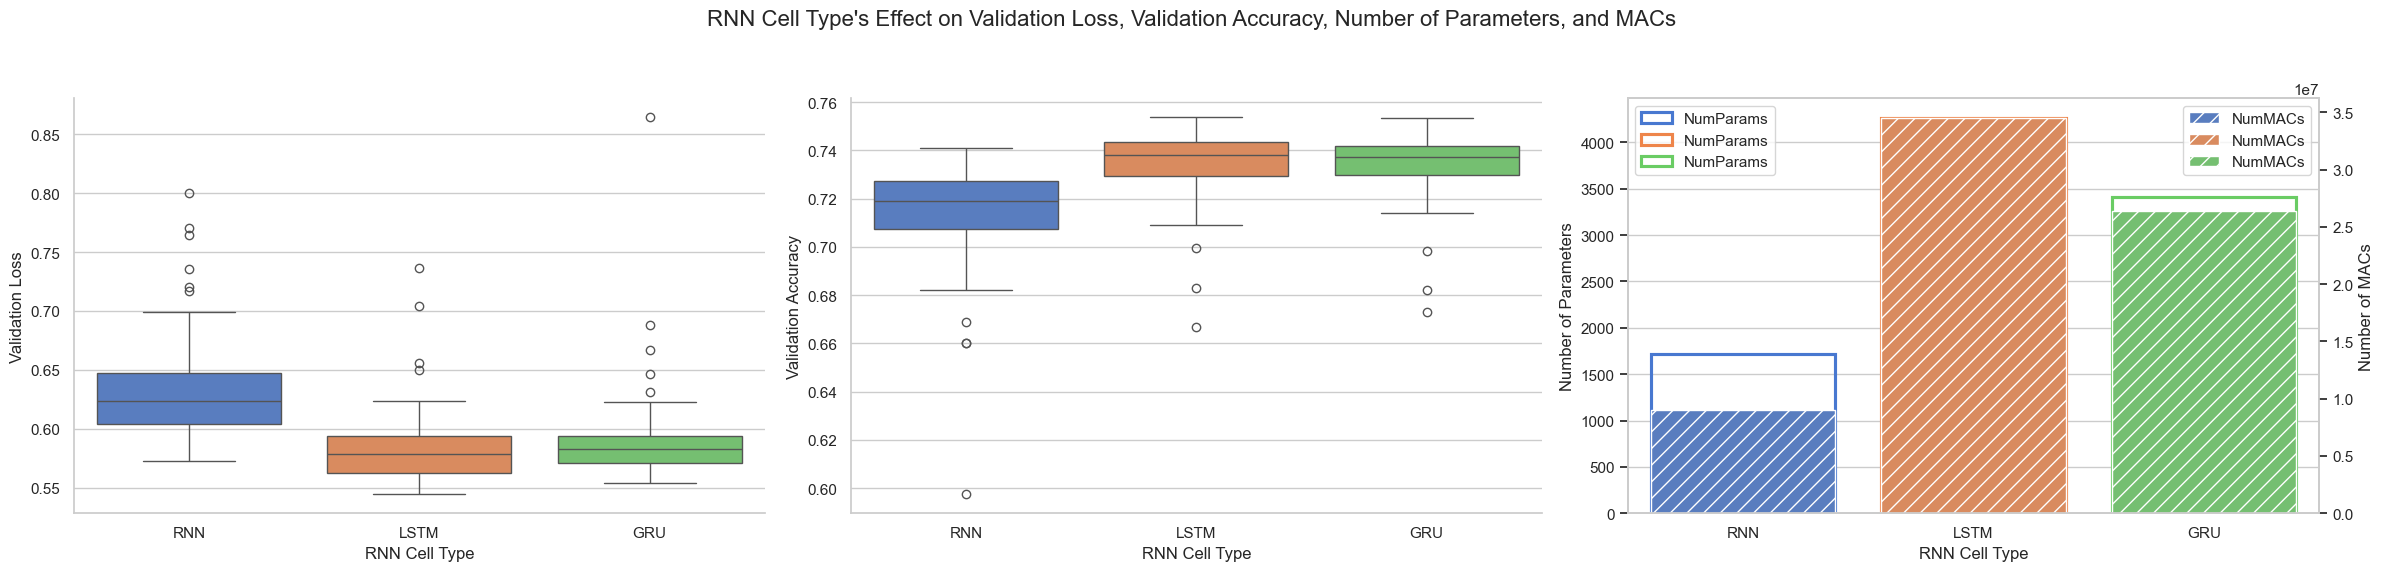
\includegraphics[width=1\textwidth]{figures/06_ModelExploration/RNN/rnn_cell_types.png}
    \caption{Comparison of RNN cell types with respect to validation loss, validation accuracy, and computational complexity.}
    \label{fig:rnn_cell_types}
\end{figure}

\begin{table}[H]
    \centering
    \caption{Comparison of Different RNN Cell Types}
    \label{tab:rnn_cell_types}
    \begin{tabular}{@{}lcccccccc@{}}
    \toprule
    & \multicolumn{2}{c}{\( \meanLossCEVal \) } & \multicolumn{2}{c}{ \( \meanAccVal \) } & \multicolumn{2}{c}{\#Params} & \multicolumn{2}{c}{\#MACs} \\
    \cmidrule(lr){2-3} \cmidrule(lr){4-5} \cmidrule(lr){6-7} \cmidrule(lr){8-9}
    RNN Cell Type & \( \nu \) & \( \%\Delta \) & \( \nu \) & \( \%\Delta \) & \( \nu \) & \( \%\Delta \) & \( \nu \) & \( \%\Delta \) \\
    \midrule
    RNN  & 0.634 & —             & 0.714 & —            & 1718 & —          & 8784  & —           \\
    GRU  & 0.591 & \gnbx{-6.72}  & 0.734 & \gnbx{2.76} & 3414 & \rdbx{98.7} & 25780 & \rdbx{193}\\
    LSTM & 0.585 & \gnbx{-7.78}  & 0.734 & \gnbx{2.84} & 4262 & \rdbx{148}  & 33700 & \rdbx{283}\\
    \bottomrule
    \end{tabular}
\end{table}

This choice is substantiated by the empirical findings presented in~\autoref{tab:rnn_cell_types} and~\autoref{fig:rnn_cell_types},
which compare the cell types based on performance and computational demands, revealing the traditional RNN cell as the most balanced option.\\
The significantly lower computational complexity of the RNN cell, compared to GRU and LSTM cells, stems from its simpler
structure without gating mechanisms. Each gate in GRU and LSTM cells—two for GRU and three for LSTM—requires its own
set of parameters and non-linear operations, specifically \( \operatorname{sigmoid} \) and \( \operatorname{tanh} \) functions.
In contrast, the traditional RNN relies on a single \( \operatorname{tanh} \) activation function, markedly reducing the
number of parameters and computational operations required.

The purpose of the gating mechanisms in GRU and LSTM cells is to manage the temporal flow of information, allowing the model to
retain or discard information as needed. This capability is particularly beneficial for long sequences with high complexity, where the
incorporation of dependencies over extended temporal horizons with varying correlations is an intricate task. Furthermore, the
vanishing gradient problem is more likely to compromise the model's ability to capture long-term dependencies.\\
However, the relatively short sequence length, determined by the number of antennas \( M \), and low complexity of our input data,
alleviate concerns related to the vanishing gradient problem or dependencies with temporal dispersion, making the traditional
RNN cell a suitable choice for the given tasks.\\

\subsubsection{Further Architectural Considerations}

The exploration of the hyperparameter space for the RNN architecture extends beyond the selection of the cell type.\\
Further architectural considerations include the sequence order, bidirectionality, and the integration of convolutional
layers for enhanced feature extraction.\\
Additionally, a fine-tuning of hyperparameters, such as the number of hidden units and learning rate was conducted. \\


\begin{figure}[H]
    \centering
    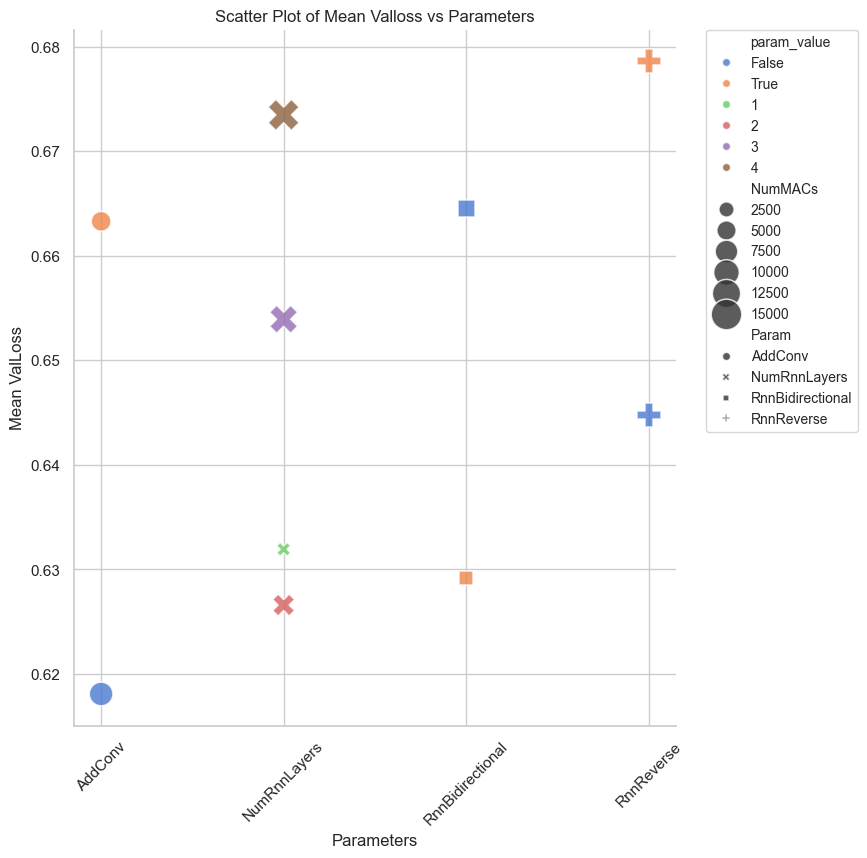
\includegraphics[width=0.6\textwidth]{figures/06_ModelExploration/RNN/rnn_scatter.png}
    \caption{Comparison of various hyperparameters with respect to the mean validation loss.}
    \label{fig:rnn_scatter}
\end{figure}

\autoref{fig:rnn_scatter} illustrates the impact of different hyperparameters on the mean validation loss \( \meanLossCEVal \) and
also aims to deliver a rather qualitative dependence of the model complexity in terms of \glspl{mac} by the marker sizes.\\
The impacts of theses architectural considerations depicted in~\autoref{fig:rnn_scatter} are furthermore gathered in~\autoref{tab:model_variants}:

\begin{table}[H]
    \centering
    \caption{Comparison of Model Variants}
    \label{tab:model_variants}
    \begin{tabular}{@{}lcccccccc@{}}
    \toprule
    & \multicolumn{2}{c}{\( \meanLossCEVal \) } & \multicolumn{2}{c}{ \( \meanAccVal \) } & \multicolumn{2}{c}{\#Params} & \multicolumn{2}{c}{\#MACs} \\
    \cmidrule(lr){2-3} \cmidrule(lr){4-5} \cmidrule(lr){6-7} \cmidrule(lr){8-9}
    Configuration & \( \nu \) & \( \%\Delta \) & \( \nu \) & \( \%\Delta \) & \( \nu \) & \( \%\Delta \) & \( \nu \) & \( \%\Delta \) \\
    \midrule[0.2pt]
    One Layer  & 0.632 &   —            &  0.717&   —            & 638  &   —           &  1830 &   —  \\
    Two Layers & 0.627 &   \gnbx{-0.844}&  0.718&   \gnbx{0.192}&  1470 &   \rdbx{130}&  6948 &   \rdbx{280}   \\
    \midrule[0.2pt]
    Without \texttt{CNNP} & 0.618 & —             & 0.724 & —             & 1287 & —       & 5308        &     — \\
    With \texttt{CNNP}    & 0.663 & \rdbx{7.31}    & 0.701  & \rdbx{-3.19}   & 1503 & \rdbx{17.6} & 8304 & \rdbx{56.4} \\
    \midrule[0.2pt]
    Unidirectional  & 0.665 & —             & 0.701 & —             & 1256 & —       & 5728 & — \\
    Bidirectional   & 0.629 & \gnbx{-5.32}   & 0.718 & \gnbx{2.34}    & 1648 & \rdbx{31.2} & 8707 & \rdbx{52.0} \\
    \midrule[0.2pt]
    Descending Order & 0.645 & —             & 0.710   & —             & 1701 & —       & 8825 & — \\
    Ascending Order  & 0.679 & \rdbx{5.24}    & 0.695 & \rdbx{-2.07}   & 1610 & — & 8624 & — \\
    \bottomrule
    \end{tabular}
\end{table}

\paragraph{Vertical Depth}
The vertical depth of an RNN refers to the number of recurrent cells stacked on top of each other to form a
deeper network architecture. Each non-final layer's output constitutes the input to the subsequent layer.\\
This concept should become clear through the consideration of~\autoref{fig:rnn_architecture}, which depicts the unrolled
architecture of the fineal RNN model. The RNN cell \( \mathrm{RNN}^{\rightarrow}_{t, 1} \) is the first layer of the RNNs
forward path, and its output is subsequently fed into the second RNN cell \( \mathrm{RNN}^{\rightarrow}_{t, 2} \). \\
Both cells exhibit their own set of weights, biases and hidden states.\\
The addition of a second RNN layer yields a marginal improvement, whereas the inclusion of further
layers causes the model to overfit on the training data. Although, the additional computational complexity introduced by
the additional layer can \emph{not} be justified by the marginal performance gain, it was unfortunately decided to utilize a
two-layered RNN architecture in the final model. \\
This decision can be attributed to an incorrect initial assessment of this hyperparameters impact on the model's performance.\\


\paragraph{Hybrid Architecture} The integration of a \texttt{CNNP} block from~\autoref{sec:cnn} was considered as an
initial feature extraction step. \\
The \texttt{CNNP}'s output \( \bfm{X} \in \mathbb{R}^{\B \times C_{\text{out}} \times 3} \) was permuted accordingly to~\autoref{eq:transposition_rnn}
and subsequently fed into the RNN. \\
However, empirical results indicated a performance detriment rather than a benefit, suggesting that direct processing of
the sequence by the RNN is more suitable.

\paragraph{Bidirectional Configuration}
The bidirectional RNN outperforms the unidirectional RNN in terms of validation loss and accuracy. \\
In a bidirectional RNN, the input sequence is processed by two separate RNN layers simultaneously—one moving
forward from the start to the end of the sequence and the other moving backward from the end to the start~\cite[Chapter 10.3]{dlbook}.
The outputs from these two layers at each time-step, capturing the respective past and future contextual information,
are combined by concatenation to form a single output that represents the full contextual understanding at
that point in the sequence.
This consolidated output is then utilized by subsequent layers in the network -- in our case, the fully connected classification head.


\paragraph{Sequence Order}
The model's performance is influenced by the order in which eigenvalues are presented in the input tensor.
Using \( \bfLT^{(\text{RNN})}_{:,::-1,:} \) to present eigenvalues in ascending order, akin to the approach of the \gls{eft} algorithm,
results in poorer performance. \\
This observation can be rationalized by considering that the most critical attributes are encapsulated within the signal
eigenvalues \( \bfL_{S} \) and their comparative magnitude relative to the smaller eigenvalues associated with noise.
By arranging the eigenvalues in descending order for input into the model, it ensures that these pivotal features are
introduced to the model at the outset. This arrangement guarantees that the RNN layers subject these significant features
to a more thorough processing over time, enhancing the model's ability to focus on and leverage these key elements for
improved performance.


\paragraph{Number of Hidden Units}
\begin{figure}[H]
    \centering
    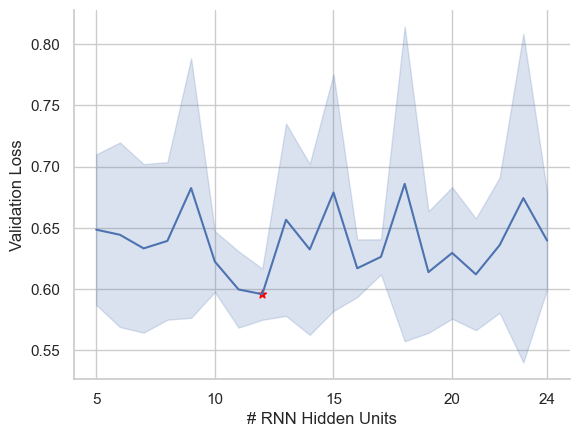
\includegraphics[width=0.5\textwidth]{figures/06_ModelExploration/RNN/rnn_num_hidden.png}
    \caption{Evaluation of the number of hidden units with respect to the mean validation loss.}
    \label{fig:rnn_hidden_units}
\end{figure}

The number of hidden units, denoted as \(H\), defines the dimensionality of the hidden state vector \(\bfm{h}_t\) at
each time step \(t\).\\
The impact of varying the number of hidden units on the mean validation loss, \(\meanLossCEVal\),
is illustrated in~\autoref{fig:rnn_hidden_units}.
A clear correlation between the number of hidden units and the mean validation loss is not evident. This observation led
to the selection of a conservative twelve hidden units -- \( \meanLossCEVal \) happens to exhibit a local minimum at this point.

The computation of the hidden state \(\bfm{h}_t\) at time step \(t\) is articulated by the following equation, which
integrates the influence of both the previous hidden state \(\bfm{h}_{t-1}\) and the current input \(\bfL_t\)~\cite{dlcheatsheet}:

\begin{equation}
    \bfm{h}_t = \operatorname{g}(\bfm{W}_{hh} \bfm{h}_{t-1} + \bfm{W}_{h\lambda} \bfL_t + \bfm{b}_h), \quad \operatorname{g} \in \{\operatorname{tanh}, \operatorname{ReLU}\}
    \label{eq:rnn_hidden_state}
\end{equation}

Here, \(\bfm{W}_{hh} \in \mathbb{R}^{H \times H}\) and \(\bfm{W}_{h\lambda} \in \mathbb{R}^{H \times M}\),
are the weight matrices, \( M \) is the dimensionality of the input vector containing the eigenvalues \( \bfL \), and
\(H\) is the number of hidden units.

\paragraph{Activation Function} The selection of non-linearities (\( g \)) for RNN cells in \textsc{PyTorch} is confined to
the \(\operatorname{tanh}\) and \(\operatorname{ReLU}\) functions. \\
The \(\operatorname{tanh}\) function has been chosen as the activation function for RNN cells, as it is the default option
for \emph{deep} RNN architectures since it tends to produce fewer dead neurons compared to the \(\operatorname{ReLU}\) function in \emph{deep} networks~\cite{lecun1998}. \\
While \(\operatorname{tanh}\) mitigates the risk of exploding gradients, \(\operatorname{ReLU}\) diminishes the likelihood of
vanishing gradients~\cite{pascanu2013difficulty}.\\
Given the shallowness of the RNN architecture, \(\operatorname{ReLU}\) might present a viable alternative to \(\operatorname{tanh}\),
and would be worth further investigation in future work.

\subsection{Resulting Architecture}

\begin{figure}[H]
    \centering
    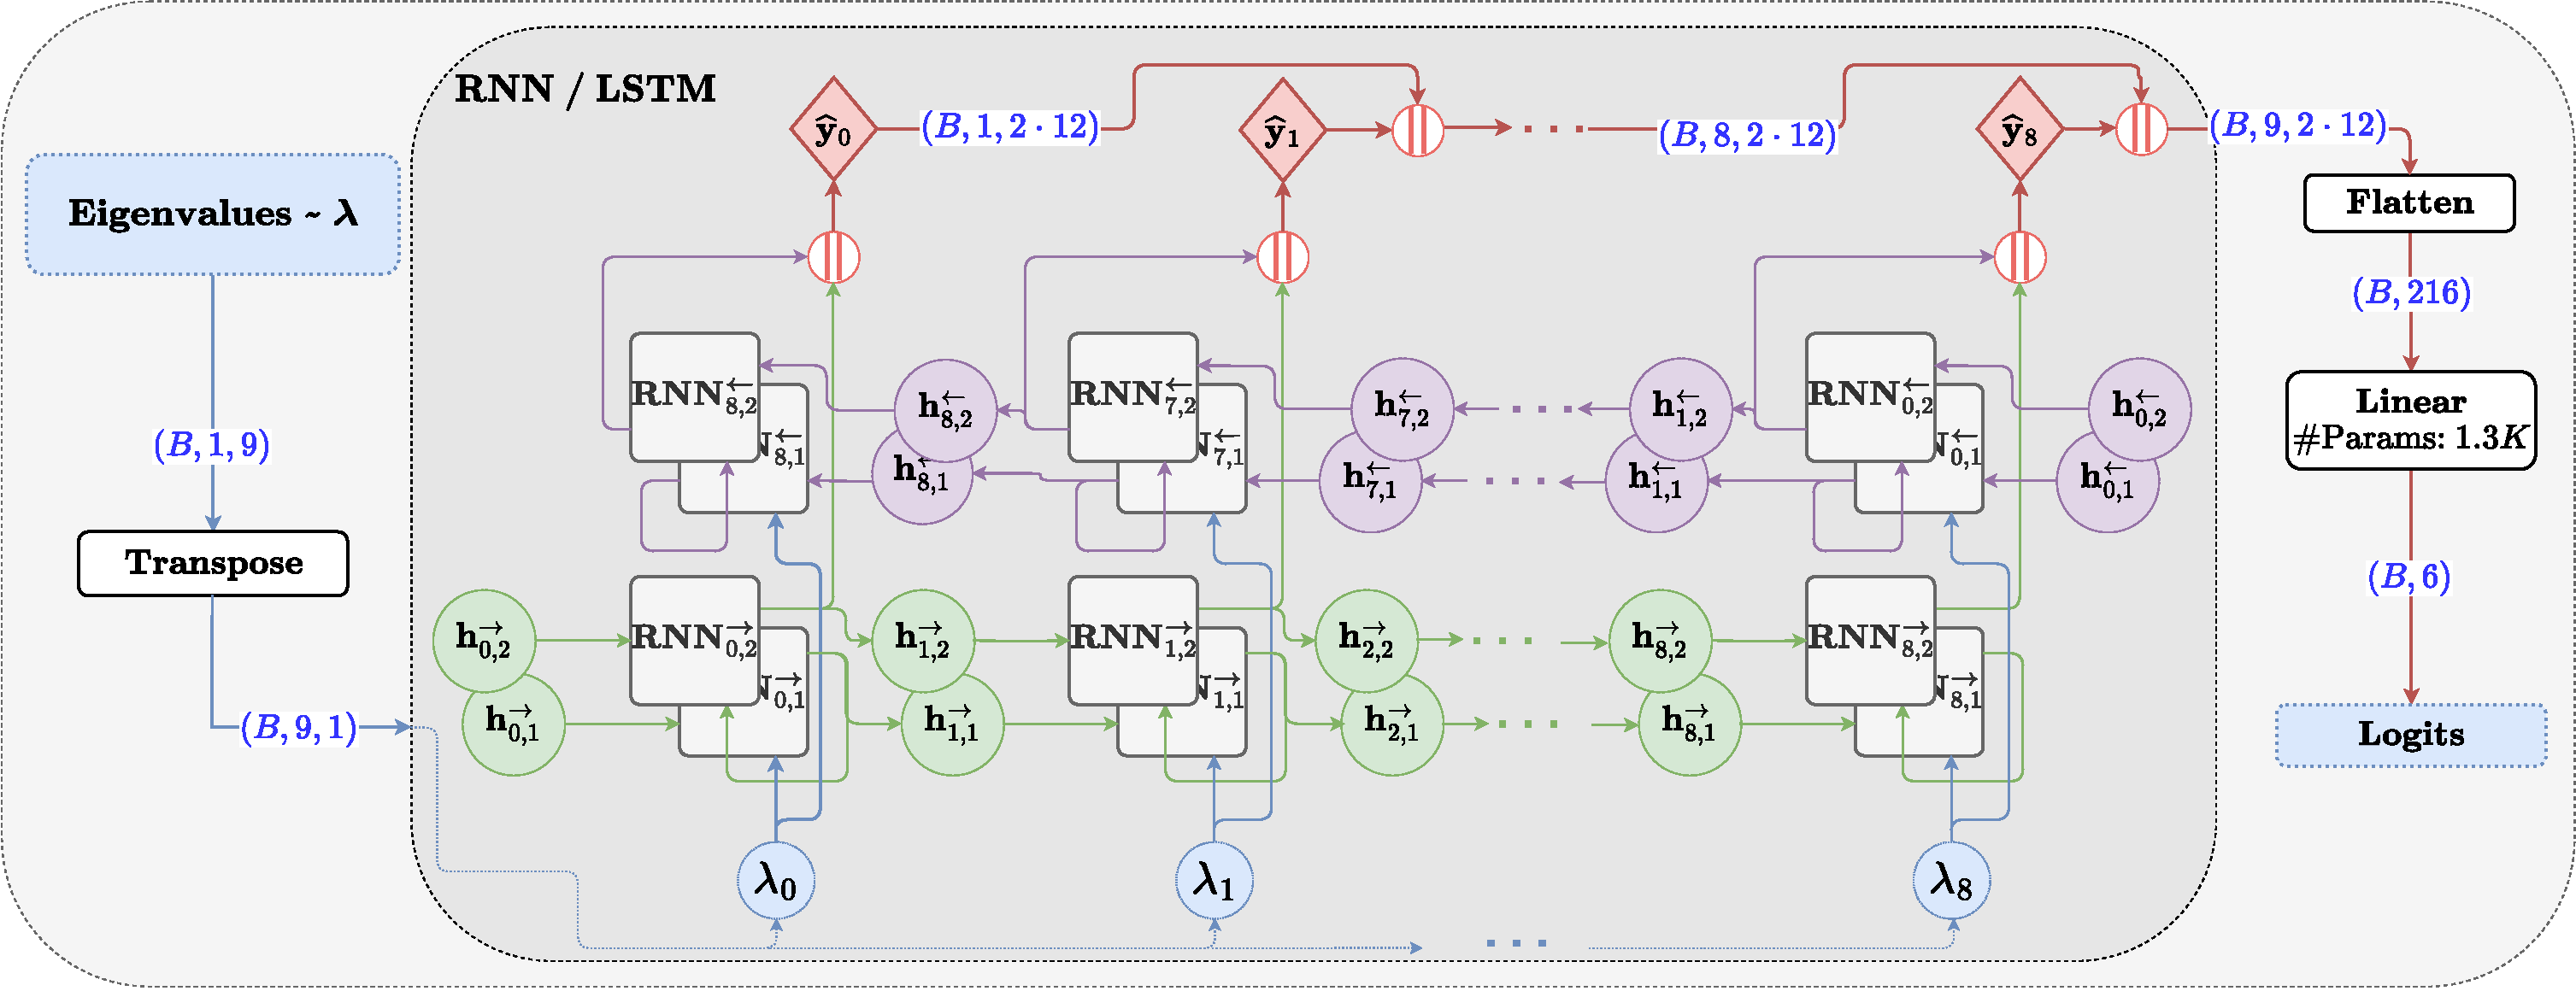
\includegraphics[width=1\textwidth]{figures/06_ModelExploration/RNN/rnn.pdf}
    \caption{Architecture of the unrolled bidirectional deep RNN.}
    \label{fig:rnn_architecture}
\end{figure}

The finalized architecture, as depicted in \autoref{fig:rnn_architecture}, embodies a deep, bidirectional RNN. \\
It leverages the capacity of bidirectional processing to capture the temporal dependencies from both forward \( \bullet^{\rightarrow} \)
and backward directions \( \bullet^{\leftarrow} \) of the input sequence.  \\
The deep structure, with two RNN layers (\( \mathrm{RNN}_{t,1} \rightarrow \mathrm{RNN}_{t,2} \)), enhances the model's
ability to abstract higher-level features, while maintaining computational efficiency.

This architecture is ``unrolled'' in the sense that it showcases each time step in the processing sequence, elucidating
the flow of data through the RNN cells. The input sequence is transposed to align the data for the bidirectional layers.\\
The RNN's output tensor has a shape of
\[
    (\B, L, D \cdot H), \quad \text{where}\: L = M, \: H = 12, \: D = \begin{cases}
                                                                    2 & \text{if bidirectional} \\
                                                                    1 & \text{otherwise.}
                                                                \end{cases}
\]
The output tensor is subsequently flattened and fed into a fully connected layer for the final classification. \\

The final model's hyperparameters and layer configurations are summarized in~\autoref{tab:rnn_summary}.
\begin{table}[H]
    \centering
    \caption{Summary of Hyperparameters and Layer Configurations for RNN Model}
    \label{tab:rnn_summary}
    \small
    \begin{tabular}{@{}lll@{}}
    \textbf{Block / Module}               & \textbf{Child}        & \textbf{Parameters / Value}            \\ \midrule
    \multicolumn{3}{l}{\textbf{Modules}}                                                     \\ \midrule
    \multirow{7}{*}{RNN Cell}
    & \texttt{nn.RNN} & Input Size: 1, Hidden Units: 12 \\
    & & Layers: 2, Bidirectional: \texttt{True}, Dropout: 0.06 \\
    & & Non-Linearity: \texttt{tanh}, \#Params: 1.3K \\
    & & \\
    & \texttt{nn.LSTM} & Input Size: 1, Hidden Units: 12 \\
    & & Layers: 2, Bidirectional: \texttt{True}, Dropout: 0.06 \\
    & & \#Params: 5.1K \\
    \midrule
    \multirow{2}{*}{Head}
    & \texttt{nn.Flatten}          &             \\
    & \texttt{nn.Linear}          & Features: \( 216 \rightarrow 6\), \#Params: 1302 \\
    \midrule[0.1pt]
    \addlinespace[0.5cm]
    \( \Sigma \) \#\(\text{Params}_{\text{RNN}}  \)               & & 2.6k\\
    \( \Sigma \) \#\(\text{Params}_{\text{LSTM}}  \)               & & 6.4k\\
    \bottomrule

    \addlinespace[1cm]
    \multicolumn{3}{l}{\textbf{Non-Layer Hyperparameters}}                                       \\ \midrule
    Optimizer                            &                           & \texttt{optim.AdamW} \\
    Batch Size                           &                           & 512                       \\
    Learning Rate                        &                           & 0.005                     \\
    Weight Decay                         &                           & 0.01685                   \\
    LR Scheduler                         &                           & \texttt{lr\_scheduler.ReduceLROnPlateau}\\
    Precision                            &                           & \texttt{32-true}     \\
    \bottomrule
    \end{tabular}%
\end{table}
The learning rate was chosen based on the results of an optimization study, as depicted in~\autoref{fig:rnn_lerning_rate}.
The dropout rate and weight decay were carried over from the \gls{cnn} architectures, and should be optimized for the RNN if
the model is to be further refined.\\

\subsubsection{Future Improvements}
\label{subsub:future_improvements_rnn}

While the current implementation utilizes all hidden states for the
final output, future versions could explore using only the last hidden state or selective slices of the sequence to
reduce the complexity of the dense layer.\\
Some units in the RNN's output layer might not carry relevant information. Especially the first units belonging to the
backward RNN might carry less relevant information that could be discarded.\\
This could be done by utilizing a pruning technique based on the resulting weights in the final layer.

Application of normalization techniques, such as layer normalization, could be beneficial to the RNN's performance, but
require a departure from the standard \texttt{nn.RNN} module to a custom implementation.\\

Without being able to provide a comprehensive analysis of the exploding or vanishing gradient problem, it is likely that
the occurrence of this issue is rather unlikely given the limited sequence length. Hence, the application of \texttt{ReLU}
as the activation function might be a viable alternative to \texttt{tanh} in future work.\\

The deployment of a deep \gls{rnn} architecture with two layers has shown a marginal improvement in performance metrics.
However, this negligible performance gain cannot be justified by the additional computational complexity.\\
Hence, it would be worthwhile to investigate the performance of a shallow \gls{rnn} architecture without having to anticipate
a significant performance loss.\\
Alternatively, the employment of a shallow \gls{gru} or \gls{lstm} architecture with an optimized number of hidden
units would be a more resource-conscious approach.\\